
\section{Policy interaction with the environment}

This section summarizes the interaction of the policy with the environment. The full interaction is shown in figure \ref{fig:agent_interaction}.

As described in previous sections the agent's actions are controlled by the agent's policy. Given an observation the policy selects actions to execute. The observations represent the environment state. They are built from the agent's camera images. The observation processing steps transform these camera images to the observation space. The policy is a neural network that takes the observation space as input and produces actions as output. 
The actions are applied to the environment. The environment processes the actions and returns a reward and a new observation.



%\newcommand{\arenaImg}[1]{\includegraphics[width=0.15\textwidth]{Bilder/image_printer_images/agent_interaction/step_#1_arena.png}}
%\newcommand{\agentImg}[1]{\includegraphics[width=0.15\textwidth]{Bilder/image_printer_images/agent_interaction/step_#1_image_from_unity.png}}
\newcommand{\preprocessedImg}[1]{\includegraphics[width=0.15\textwidth]{Bilder/image_printer_images/agent_interaction/step_#1.png}}
\newcommand{\observationStack}{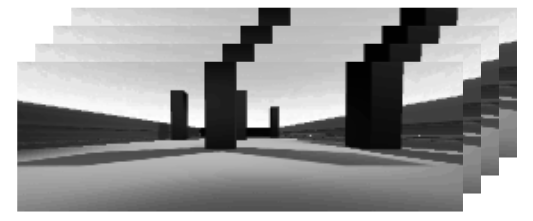
\includegraphics[width=0.15\textwidth]{Bilder/observation_stack.png}}

%\newcommand{\python}{
\includegraphics[width=0.15\textwidth]{Bilder/agent_interaction/python.png}}
%\newcommand{\unity}{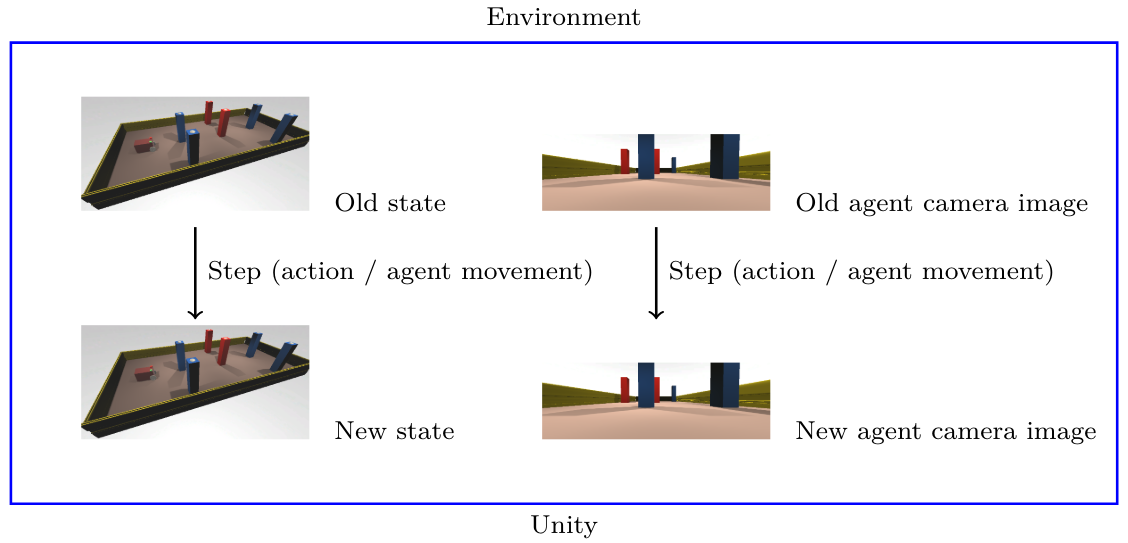
\includegraphics[width=0.15\textwidth]{Bilder/agent_interaction/unity.png}}

\newcommand\yOffsetHalf{-4}
\newcommand\yOffset{-8}

\newcommand\xOffset{0.5}

%\newcommand\envWidth{12}

\usetikzlibrary{fit}
\begin{figure}[!h]
    \centering
    \begin{tikzpicture}[%
            every node/.style={
                    font=\scriptsize,
                    % Better alignment, see https://tex.stackexchange.com/questions/315075
                    text height=1ex,
                    text depth=.25ex,
                },
        ]

        \node[fit={(0,0) (0 + \envWidth, - 5)}, inner sep=0pt, draw=blue, thick] (env) {};
        \node[above] (envText) at (env.north) {Environment};
        \node[below] (envU) at (env.south) {Unity};

        \node[above] (oldState) at (2, -2)
        {\arenaImg{0}};
        \node[right] at (oldState.east) {old state};

        \node[below] (newState) at (2, -4)
        {\arenaImg{1}};
        \node[right] at (newState.east) {new state};


        \node[above] (oldImg) at (7, -2)
        {\agentImg{0}};
        \node[right] at (oldImg.east) {old agent camera image};

        \node[below] (newImg) at (7, -4)
        {\agentImg{1}};
        \node[right] at (newImg.east) {new agent camera image};
        
        
        \draw[->,thick] (2, -2)--(2, -3);
        \node[right] at (2, -2.5) {step (action / agent movement)};

        \draw[->,thick] (7, -2)--(7, -3);
        \node[right] at (7, -2.5) {step (action / agent movement)};



        % bottom half:

        \node[fit={(0 + \xOffset,0+ \yOffset) (3+ \xOffset,-5 + \yOffset)}, inner sep=0pt, draw=blue, thick] (preprocessing) {};
        \node[above] at (preprocessing.north) {Preprocessing};
        \node[below] at (preprocessing.south) {Python};
        \node[below] (preproAgent) at (1.5+ \xOffset, -1+ \yOffset) {\agentImg{1}};
        \node[below] at (preproAgent.south) {agent camera image};
        \node[below] (preproFinish) at (1.5+ \xOffset, -4+ \yOffset) {\preprocessedImg{1}};
        \node[below] at (preproFinish.south) {preprocessed image};
        \draw[->,thick] (1.5+ \xOffset, -2+ \yOffset)--(1.5+ \xOffset, -3+ \yOffset);


        \node[fit={(4+ \xOffset,0+ \yOffset) (7+ \xOffset,-5+ \yOffset)}, inner sep=0pt, draw=blue, thick] (memory) {};
        \node[above] at (memory.north) {Memory Mechanism};
        \node[below] at (memory.south) {Python};
        \node[below] (memPre) at (5.5+ \xOffset, -1+ \yOffset) {\preprocessedImg{1}};
        \node[below] at (memPre.south) {preprocessed image};
        \node[below] (memStack) at (5.5+ \xOffset, -4+ \yOffset) {\observationStack};
        \node[below] at (memStack.south) {observation};
        \draw[->,thick] (5.5+ \xOffset, -2+ \yOffset)--(5.5+ \xOffset, -3+ \yOffset);


        \draw[decorate,decoration={brace,mirror,amplitude=5pt}] (0+ \xOffset,-5.5+ \yOffset) -- (7+ \xOffset,-5.5+ \yOffset)
        node[anchor=north,midway,below=4pt] {Observation Preprocessing};

        \node[fit={(8+ \xOffset,0+ \yOffset) (11+ \xOffset,-5+ \yOffset)}, inner sep=0pt, draw=blue, thick] (policy) {};
        \node[above] (policyText) at (policy.north) {Neural Network};
        \node[below] (policyP) at (policy.south) {Python};

        \node[below] (pObs) at (9.5+ \xOffset, -1+ \yOffset) {\observationStack};
        \node[below] at (pObs.south) {observation};

        \node[below] (pAction) at (9.5+ \xOffset, -4+ \yOffset) {Action};
        \draw[->,thick] (9.5+ \xOffset, -2 + \yOffset)--(9.5+ \xOffset, -3+ \yOffset);

        \draw[decorate,decoration={brace,mirror,amplitude=5pt}] (8+ \xOffset,-5.5+ \yOffset) -- (11+ \xOffset,-5.5+ \yOffset)
        node[anchor=north,midway,below=4pt] {Policy};

        \draw[->,thick] (3+ \xOffset, -2.5+ \yOffset)--(4+ \xOffset, -2.5+ \yOffset);
        \draw[->,thick] (7+ \xOffset, -2.5+ \yOffset)--(8+ \xOffset, -2.5+ \yOffset);


        % arrows communication
        \draw[->,thick, red] (\xOffset + 11, -2.5+ \yOffset)--(\xOffset+11+1, -2.5+\yOffset)--(\xOffset+11+1, -2.5)--(\envWidth, -2.5);
        \node[centered, fill=white] at (\envWidth +0.5, -2.5 + \yOffsetHalf) {action};

        \draw[->,thick, red] (0, -2.5)--(-0.5,-2.5)--(-0.5,-2.5+\yOffset)--(\xOffset, -2.5+ \yOffset);
        \node[right] (camArrow) at (-2, -2.5 + \yOffsetHalf) {\agentImg{1}};
        
        \node[below, fill=white] at (camArrow.south) {rewards + new agent camera image};

    \end{tikzpicture}
    \caption{Full policy interaction with the environment, communication in red}
    \label{fig:agent_interaction}
\end{figure} % this replaces the old rl_cycle image
